\documentclass{asaproc}
%\documentclass{article}
\usepackage{amssymb,amsmath,amsthm}
\usepackage{graphicx}
%\usepackage[ruled,linesnumbered]{algorithm2e}
\usepackage[caption = false]{subfig}
\usepackage{float}

%\usepackage{times}
%If you have times installed on your system, please
%uncomment the line above

%For figures and tables to stretch across two columns
%use \begin{figure*} \end{figure*} and
%\begin{table*}\end{table*}
% please place figures & tables as close as possible
% to text references

% Commands
\newcommand{\sq}{\sigma^2}
\newcommand{\tq}{\tau^2}
\newcommand{\laq}{\lambda^2}
\newcommand{\bh}{\hat{\beta}}
\newcommand{\Sh}{\hat{\Sigma}}

% Figures Path
\graphicspath{{./figures/}}

\title{Defending Against Adversarial Attacks}

%input all authors' names

\author{Keller Jordan, Rene Gutierrez \& Brett G\"{o}hre \\}

%input affiliations

%{USDA Forest Service Forest Products Laboratory}

\begin{document}

\maketitle


\begin{abstract}
	
Adversarial attacks have been a growing concern as the success of Neural Networks increases. Of particular interest, are attacks that can devised without knowing the particular model used, but only the data distribution, the so called Black Box attacks. In this project we test several ideas to fend off Black Box attacks, Random Compression Matrices, and Capsule Networks with Reconstruction Error based detection.
	
\begin{keywords}
Adversarial Examples, Black-Box Attacks, Random Projection Matrix, Reconstruction Error, Capsule Networks, Convolutional Neural Networks.
\end{keywords}
\end{abstract}


\section{Introduction}

There is an increasing concern that Neural Networks are very susceptible to Black Box Adversarial Attacks, with implications that go from identity theft, as in biometrics recognition to safety in the self-driving car industry. So it is of the utmost importance to try to create defenses against such attacks, or at the very least study their characteristics. Here we try several alternatives with varying degrees of success, however even in failure, new insights are gained in exploration.

\section{Random Projection Matrices}

\subsection*{Idea}

Random compression matrices have been found to be able to perform dimensionality reduction exploiting the input data structure, in particular when the data could belong to a manifold. We can make further use of this in two ways, first the dimensionality reduction can help create smaller models that could help robustness. Furthermore, the random nature of the matrix can transform the attack and make it less or not powerful at all.

\subsection*{Method}

For this idea we worked with the MNIST dataset. First, we created 2 sets of adversarial examples based on different architectures. The first set was based on Logistic Regression and consists of 758 adversarial images. The second one was based on a Convolutional Neural Network optimized to 95\% accuracy in the validation set, and had 440 adversarial images. Then we tried to attack these architectures plus a Random Compression Matrix architecture, a Random Expansion Matrix and 2 CNN optimized to 90\% and 99\% accuracy.

The Random Projection architectures where basically a Logistic Regression for which a Random Projection Matrix $ \Phi $ is applied to the input $ x $, but remains fixed through training. The idea was that since adversarial attacks are based on small perturbations $ \epsilon $ to the input, then when applying the random matrix the perturbation would be rendered meaningless, that is $ \Phi \epsilon $ would not be able to attack as effectively. Furthermore, since the attacker would not know $ \Phi $, it would not be able to train attacks specific to it. In this way our random projection matrix can be thought as some kind of code.

\begin{figure}[h!]
	\centering
	\caption{\enspace Examples of the Adversarial Attacks created under the 2 Architectures. The top row shows the attacks created with the Logistic Regression, while the bottom was created using a CNN.}
	\subfloat[Adversarial Attack for 3]{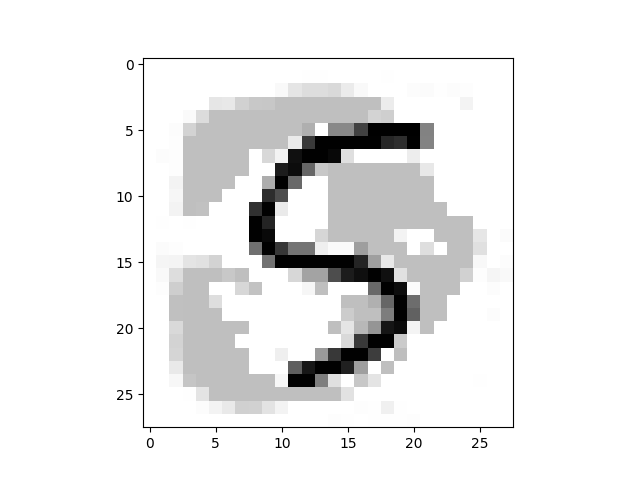
\includegraphics[width=0.45\linewidth]{advImg.png}} 
	\subfloat[Noise  ]{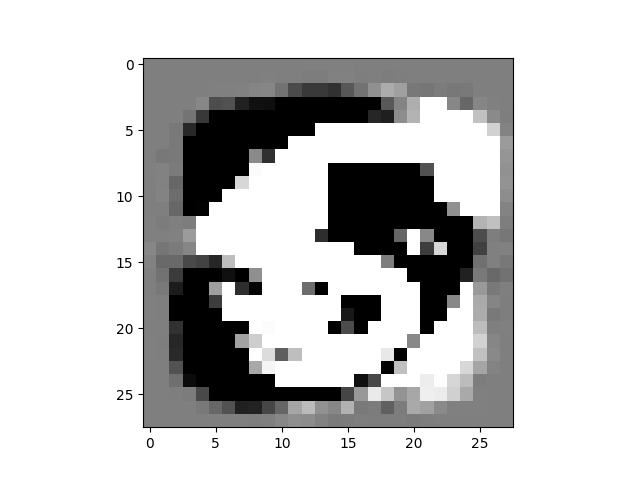
\includegraphics[width=0.45\linewidth]{advNoi.png}}   \\
	\subfloat[Adversarial Attack for 3]{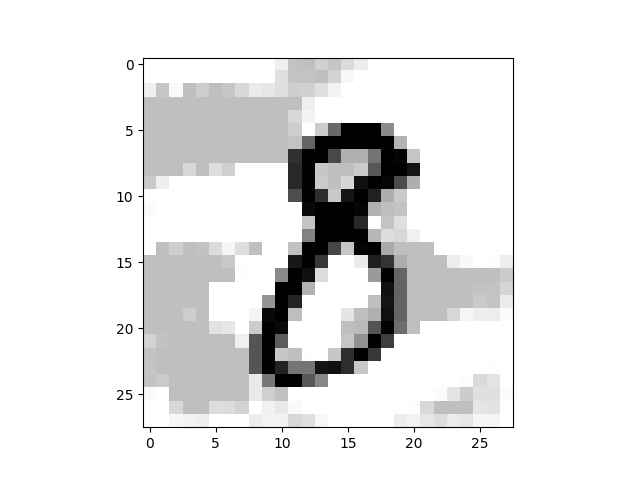
\includegraphics[width=0.45\linewidth]{advImgCnn.png}} 
	\subfloat[Noise  ]{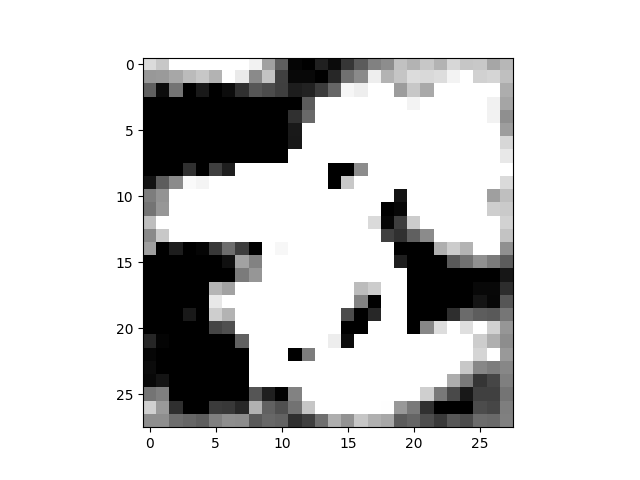
\includegraphics[width=0.45\linewidth]{advNoiCnn.png}}   \\
	\label{fig1}
\end{figure}


\subsection*{Results}

\begin{table*}
	\caption{\enspace Accuracy for the 5 different methods, using the test set and the adversarial examples generated by Logistic Regression and CNN architectures.}
	\label{tab1}
	\begin{tabular*}{\hsize}{@{\extracolsep{\fill}}cccc}
		\hline
		\\[-7pt]
		\multicolumn{1}{c}{\it Method}                    & 
		\multicolumn{1}{c}{\it Test Set}                  & 
		\multicolumn{1}{c}{\it Logistic Arch Adversarial} & 
		\multicolumn{1}{c}{\it CNN Arch Adversarial}      \\
		\hline
		\\[-5pt]
		Logistic Regression      & 92.00\% & 0.00\%  & 3.41\%  \\
		CNN 90\%                 & 89.82\% & 8.71\%  & 5.23\%  \\
		CNN 95\%                 & 94.64\% & 9.50\%  & 9.50\%  \\
		CNN 99\%                 & 98.63\% & 60.95\% & 11.36\% \\
		Compression Logistic to 196 dim & 89.56\% & 0.00\%  & 5.00\%  \\
		Expansion Logistic to 1960 dim  & 91.07\% & 0.00\%  & 3.64\% 
	\end{tabular*}
\end{table*}

\begin{figure}[h!]
	\centering
	\caption{\enspace Confusion Matrices for the True Target and Predicted Target on the Left and the Adversarial Target and Predicted Target on the Right. The top row shows the results using the a compression matrix, while the bottom row shows the results on an expansion matrix. Both results are for the adversarial examples generated with the Logistic Regression architecture.}
	\subfloat[Confusion Matrix for True Class]{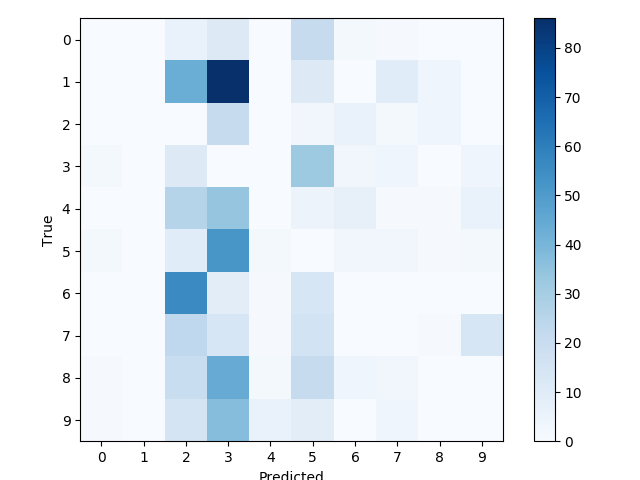
\includegraphics[width=0.5\linewidth]{confussionMatrixAdvTrueCom.png}} 
	\subfloat[Confusion Matrix for Target Class]{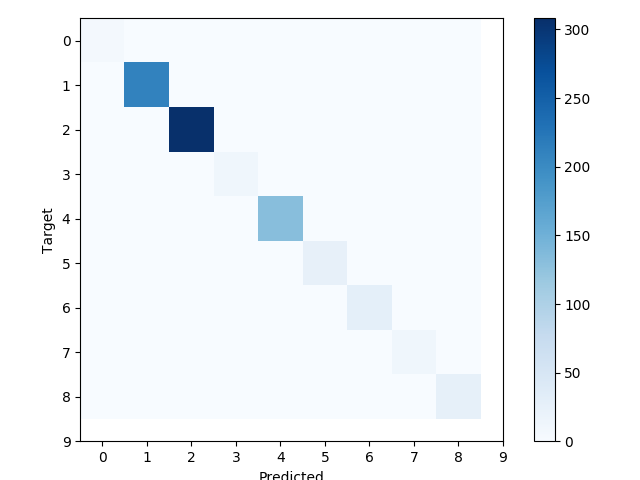
\includegraphics[width=0.5\linewidth]{confussionMatrixAdvTarCom.png}}   \\
	\subfloat[Confusion Matrix for True Class]{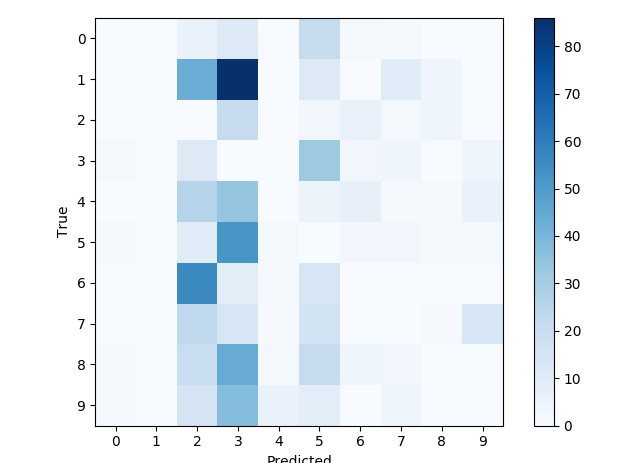
\includegraphics[width=0.5\linewidth]{confussionMatrixAdvTrueExp.png}} 
	\subfloat[Confusion Matrix for Target Class]{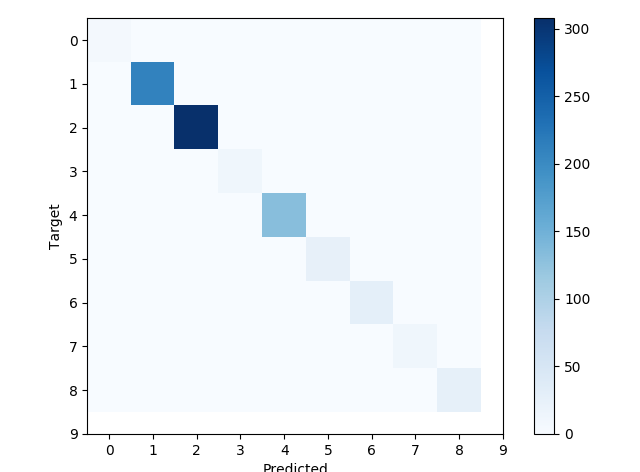
\includegraphics[width=0.5\linewidth]{confussionMatrixAdvTarExp.png}}   \\
	\label{fig2}
\end{figure}

In figure \ref{fig2} we can see the corresponding confusion matrices for the true class on the left and for the adversarial class on the right for the examples generated from the Logistic regression architecture. As we can see the adversarial attacks not only make the expansion and compression defenses fail to predict correctly, but are completely fooled by the examples.

Furthermore, in table \ref{tab1} we can see that the adversarial examples generated by different architectures transfer successfully across architectures. Even fooling completely the randomness induced by the projecting matrices. However it seems that training the CNN to until it achieves higher accuracy provides the best protection, however it still performs poorly and offers little protection for examples generated on the CNN.

To analyze the weights obtained after compression and expansion, and compared them to the weights obtained under regular logistic regression, we apply the pseudo inverse of the projection matrix $ \Phi^+ $. In figure \ref{fig4} we can see the weights re-expanded or re-compressed to the original size. The weights for the Expansion weights are very close to the regular weights, so it comes as no surprise that the Expansion Logistic Regression fails to defend against adversarial attacks. However, even though the weights from the Compressed Logistic are significantly different this did not prevent it from getting fooled. Also, the weights seem to converge to the regular weights as the level of compression decreases, as we can see in figure \ref{fig5}, giving us a hint of why the network still gets fooled.

\begin{figure}[h!]
	\centering
	\caption{\enspace Weights for "Neuron 2", for the Compression, Expansion and Regular Logistic Regression.}
	\subfloat[Compression]{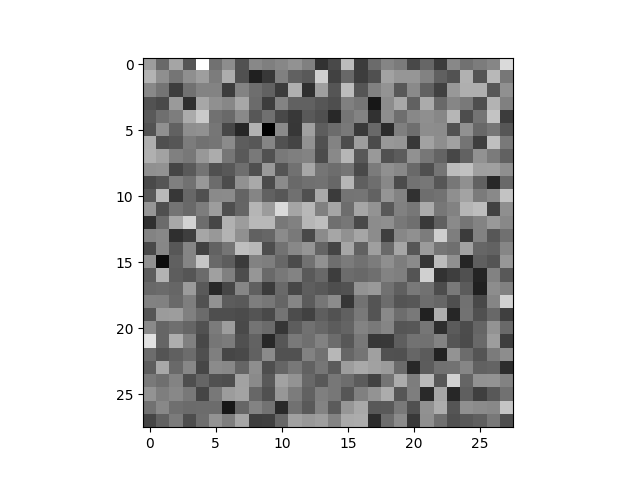
\includegraphics[width=0.33\linewidth]{com2.png}}
	\subfloat[Expansion]{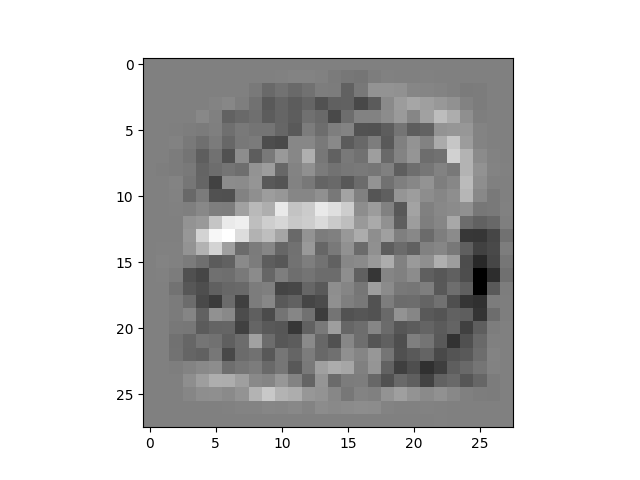
\includegraphics[width=0.33\linewidth]{exp2.png}}
	\subfloat[Regular]{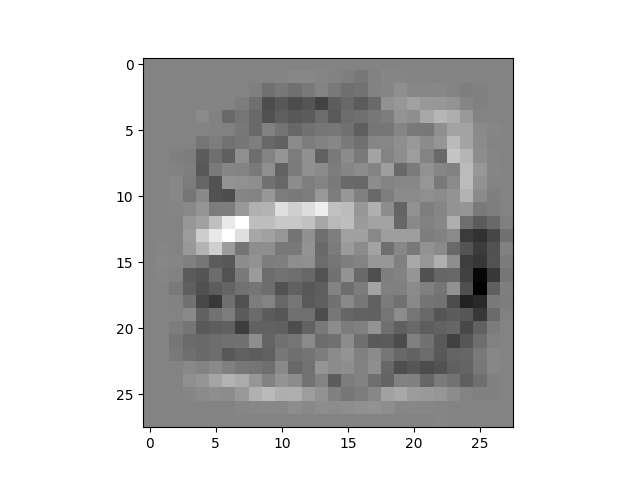
\includegraphics[width=0.33\linewidth]{reg2.png}}
	\label{fig4} 
\end{figure}

\begin{figure}[h!]
	\centering
	\caption{\enspace Weights for 2, for the Compression t0 196, Compression to 392, Compression to 588 and Regular Logistic Regression.}
	\subfloat[196]{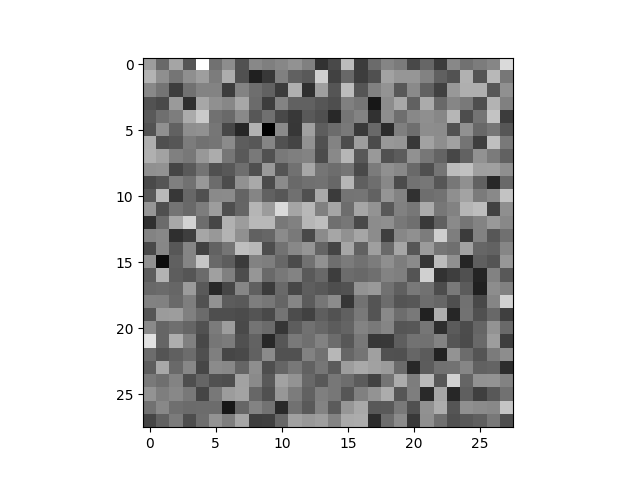
\includegraphics[width=0.25\linewidth]{com2.png}}
	\subfloat[392]{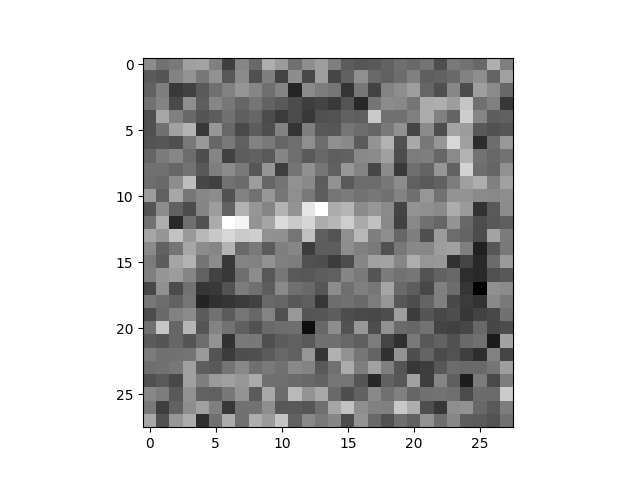
\includegraphics[width=0.25\linewidth]{co22.png}}
	\subfloat[588]{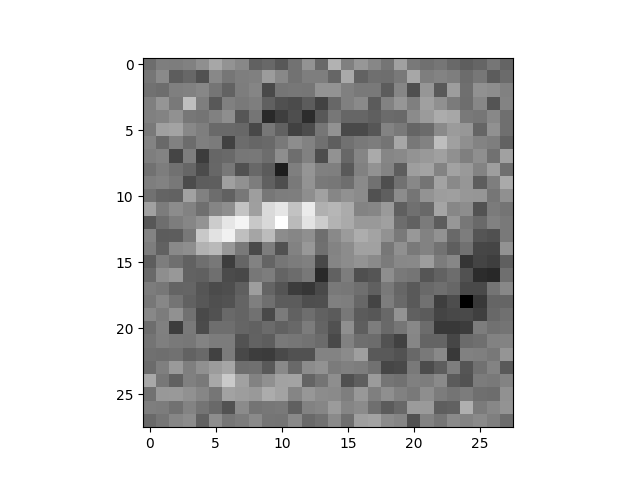
\includegraphics[width=0.25\linewidth]{co32.png}}
	\subfloat[Reg]{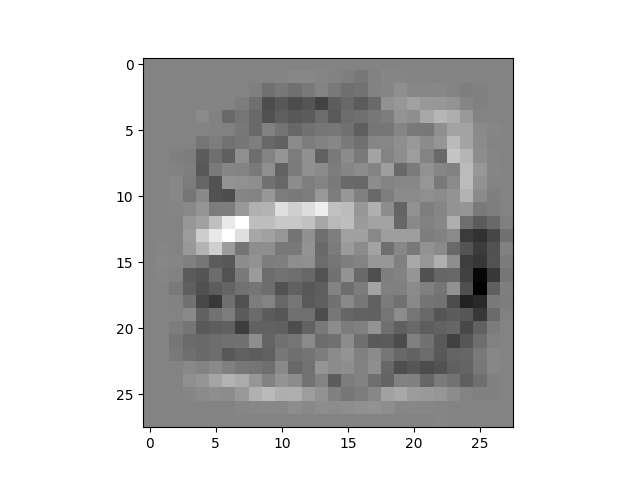
\includegraphics[width=0.25\linewidth]{reg2.png}}  
	\label{fig5} 
\end{figure}

\section*{GD vs ED}

\subsection*{Idea}

Using the square loss results accommodates Gradient Descent methods as a good iterative optimization methods, resulting on an updating rule given by:
$$ w_{t+1} \dot{=} w_t - \eta \nabla L(w_t). $$
However using the relative entropy loss results in an iterative process called Exponential Gradient, with updating rule given by:
$$ w_{t+1} \dot{=} w_t e^{-\eta \nabla L(w_t)}. $$
In this way we propose using different iterative optimization updates or different losses that could be unknown to the attacker to defend against adversarial attacks generated with the most commonly used square loss.

\subsection*{Method}

Again we generate adversarial examples based on a fully connected neural network with 2 layers of size 100 and 10, using GD and EG± on MNIST. Then we generated   adversarial attacks using to methods; Gradient Ascent (GA) and Fast Gradient Sign (FGS). 

\begin{figure}
	\centering
	\caption{\enspace Adversarial Attacks examples for the SGD on the Center and EG on the right. On the left, we have the true input, and we show the added perturbation next to each adversarial attack.}
	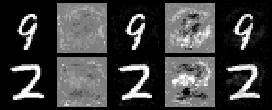
\includegraphics[width=\linewidth]{mnist_attacks.png}
	\label{fig6}
\end{figure}

\subsection*{Results}

In table \ref{tab2} we can see that generating adversarial attacks is harder for for EG than SGD. Since as the number of iterations increases the magnitude of the perturbation increases, then not only is more computationally expansive, but is easier to observe the perturbation. Again, we can observe this phenomena in figure \ref{fig6}, where the perturbation is clearly bigger for the EG examples.

\begin{table}
	\caption{\enspace Number of iterations that it takes to fool the two different optimizers SGD and EG.}
	\label{tab2}
	\begin{tabular*}{\hsize}{@{\extracolsep{\fill}}ccc}
		\hline
		\\[-7pt]
		\multicolumn{1}{c}{\it Method/Optimizer} & 
		\multicolumn{1}{c}{\it SGD}              & 
		\multicolumn{1}{c}{\it EG}               \\ 
		\hline
		\\[-5pt] 
		Gradient Ascent    & $60.9 (\pm 32.3)$ & $85.1 (\pm 40.5)$ \\ 
		Fast Gradient Sign & $52.0 (\pm 26.1)$ & $91.0 (\pm 43.5)$
	\end{tabular*}
\end{table}

\begin{figure}
	\centering
	\caption{\enspace Average perturbation to fool a 3. SGD on the Left and EG on the Right.}
	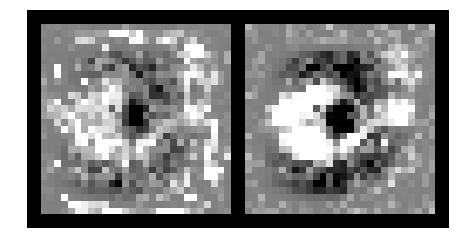
\includegraphics[width=\linewidth]{avg_attack_3.png}
	\label{fig7}
\end{figure}

Additionally in figure \ref{fig7} we can observe that on average 'fooling' an EG trained FC network requires bigger, but also more structured perturbations. As we can see in the image, it is easy to see that a 3 is captured by the EG perturbation.

\begin{table}
	\caption{\enspace Percentage of successful attacks with examples created from one optimizer to th other. Attacks generated with 200 iterations.}
	\label{tab3}
	\begin{tabular*}{\hsize}{@{\extracolsep{\fill}}ccc}
		\hline
		\\[-7pt]
		\multicolumn{1}{c}{\it Method/ Src$\to$Dst} & 
		\multicolumn{1}{c}{\it SGD$\to$EG}          & 
		\multicolumn{1}{c}{\it EG$\to$SGD}          \\ 
		\hline
		\\[-5pt] 
		Gradient Ascent     & 67.4\% & 99.0\% \\
		Fast Gradient Sign  & 88.2\% & 99.8\%
	\end{tabular*}
\end{table}

Finally, in table \ref{tab3} we can see that attacks generated with the same number of iterations transfer better from EG to SGD than the other way around. Frustratingly, both sets of attacks transfer successfully to the other optimizer. 

\section*{Detection of Adversarial Examples using Reconstruction Error}

\subsection*{Idea}

In the paper introducing Capsule Networks [https://arxiv.org/abs/1710.09829], the capsule network is trained alongside a separate network that attempts to reconstruct the input image from the vector output. The L2 distance between the original image and reconstruction is then added to the loss function and used to train both networks.

When the network is fooled by an adversarial example, the reconstruction produced by the final vector is extremely far from the input image. As a result, it should be possible to use high reconstruction loss as a linear classifier to discern between real inputs and adversarial examples.

\subsection*{Method}

We created a Capsule Network to perform reconstruction. The structure of the network can be observed in figure \ref{fig7}. Using the output reconstruction we compute the Mean Square Error between the original input and the reconstruction. Our hope is that adversarial attacks will have reconstructions that will be more different than the non adversarial ones.

\begin{figure}[h!]
	\centering
	\caption{\enspace Capsule Network Architecture}
	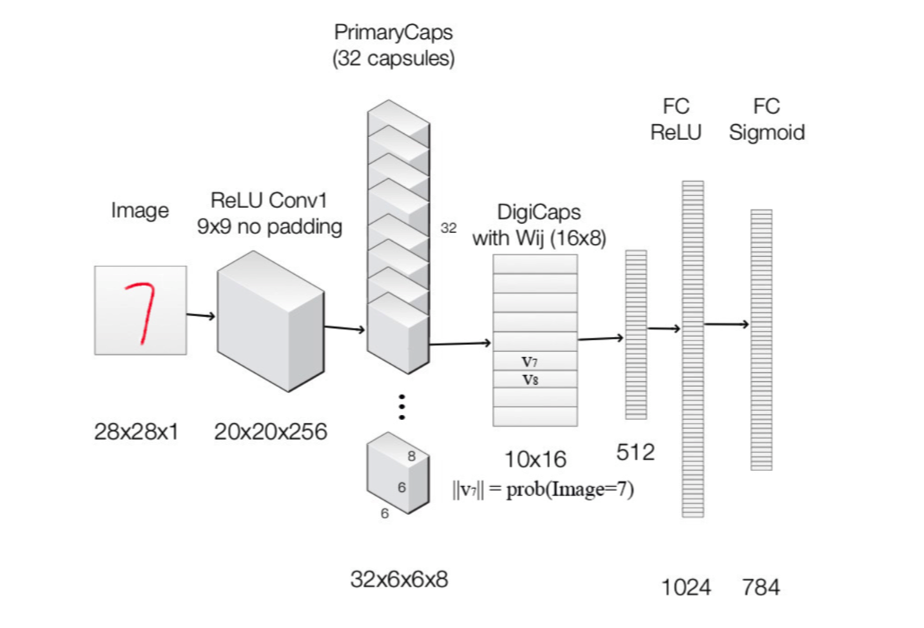
\includegraphics[width=\linewidth]{caps_recon}
	\label{fig3}
\end{figure}

In figure \ref{fig8} we can observe such examples. As we can see the reconstruction for non adversarial attacks seems closer than the adversarial reconstruction. In fact the adversarial reconstruction is a different number. The adversarial reconstruction is not always the same, as we can see in figure \ref{fig9}, the reconstruction for adversarial ones gets reconstructed as 2 or 7 in this particular examples.

\begin{figure}[h!]
	\centering
	\caption{\enspace Reconstruction Examples. Non adversarial on the Left and adversarial on the right.}
	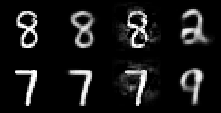
\includegraphics[width=\linewidth]{recon-fig5}
	\label{fig8}
\end{figure}

\begin{figure}[h!]
	\centering
	\caption{\enspace Reconstruction Examples. Non adversarial on the Left and adversarial on the right.}
	\subfloat[Reconstructed to 2]{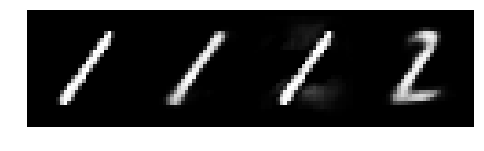
\includegraphics[width=\linewidth]{recon-fig4}} \\
	\subfloat[Reconstructed to 7]{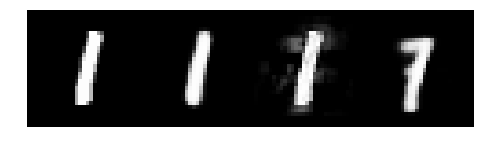
\includegraphics[width=\linewidth]{recon-fig3}}
	\label{fig9}
\end{figure}

\subsection*{Results}

In figure \ref{fig10} we can observe the ROC for attack detection. Surprisingly, we can detect around 75\% of the attacks while incurring in a 5\% false positive rate, which is a promising result that could get better with finer tune-up.

\begin{figure}[h!]
	\centering
	\caption{\enspace Receiving Operating Characteristic Curve for attack detection using different thresholds of MSE.}
	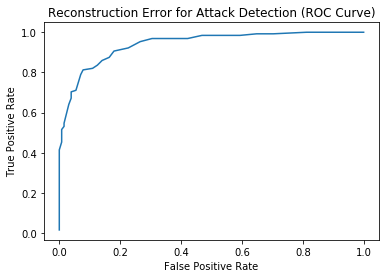
\includegraphics[width=\linewidth]{mse_roc}
	\label{fig10}
\end{figure}

%\bibliographystyle{apalike}
%\bibliography{references.bib}

\section*{Bibliography}

Sara Sabour, Nicholas Frosst, and Geoffrey E Hinton. \textit{Dynamic routing between capsules}. In
Advances in Neural Information Processing Systems, pp. 3859–3869, 2017.

Kivinen, J \& Warmuth, M (1997). \textit{Additive versus exponentiated gradient updates for linear
prediction}. Journal of Tnformation and Computation 132, 1-64. 


\end{document}




